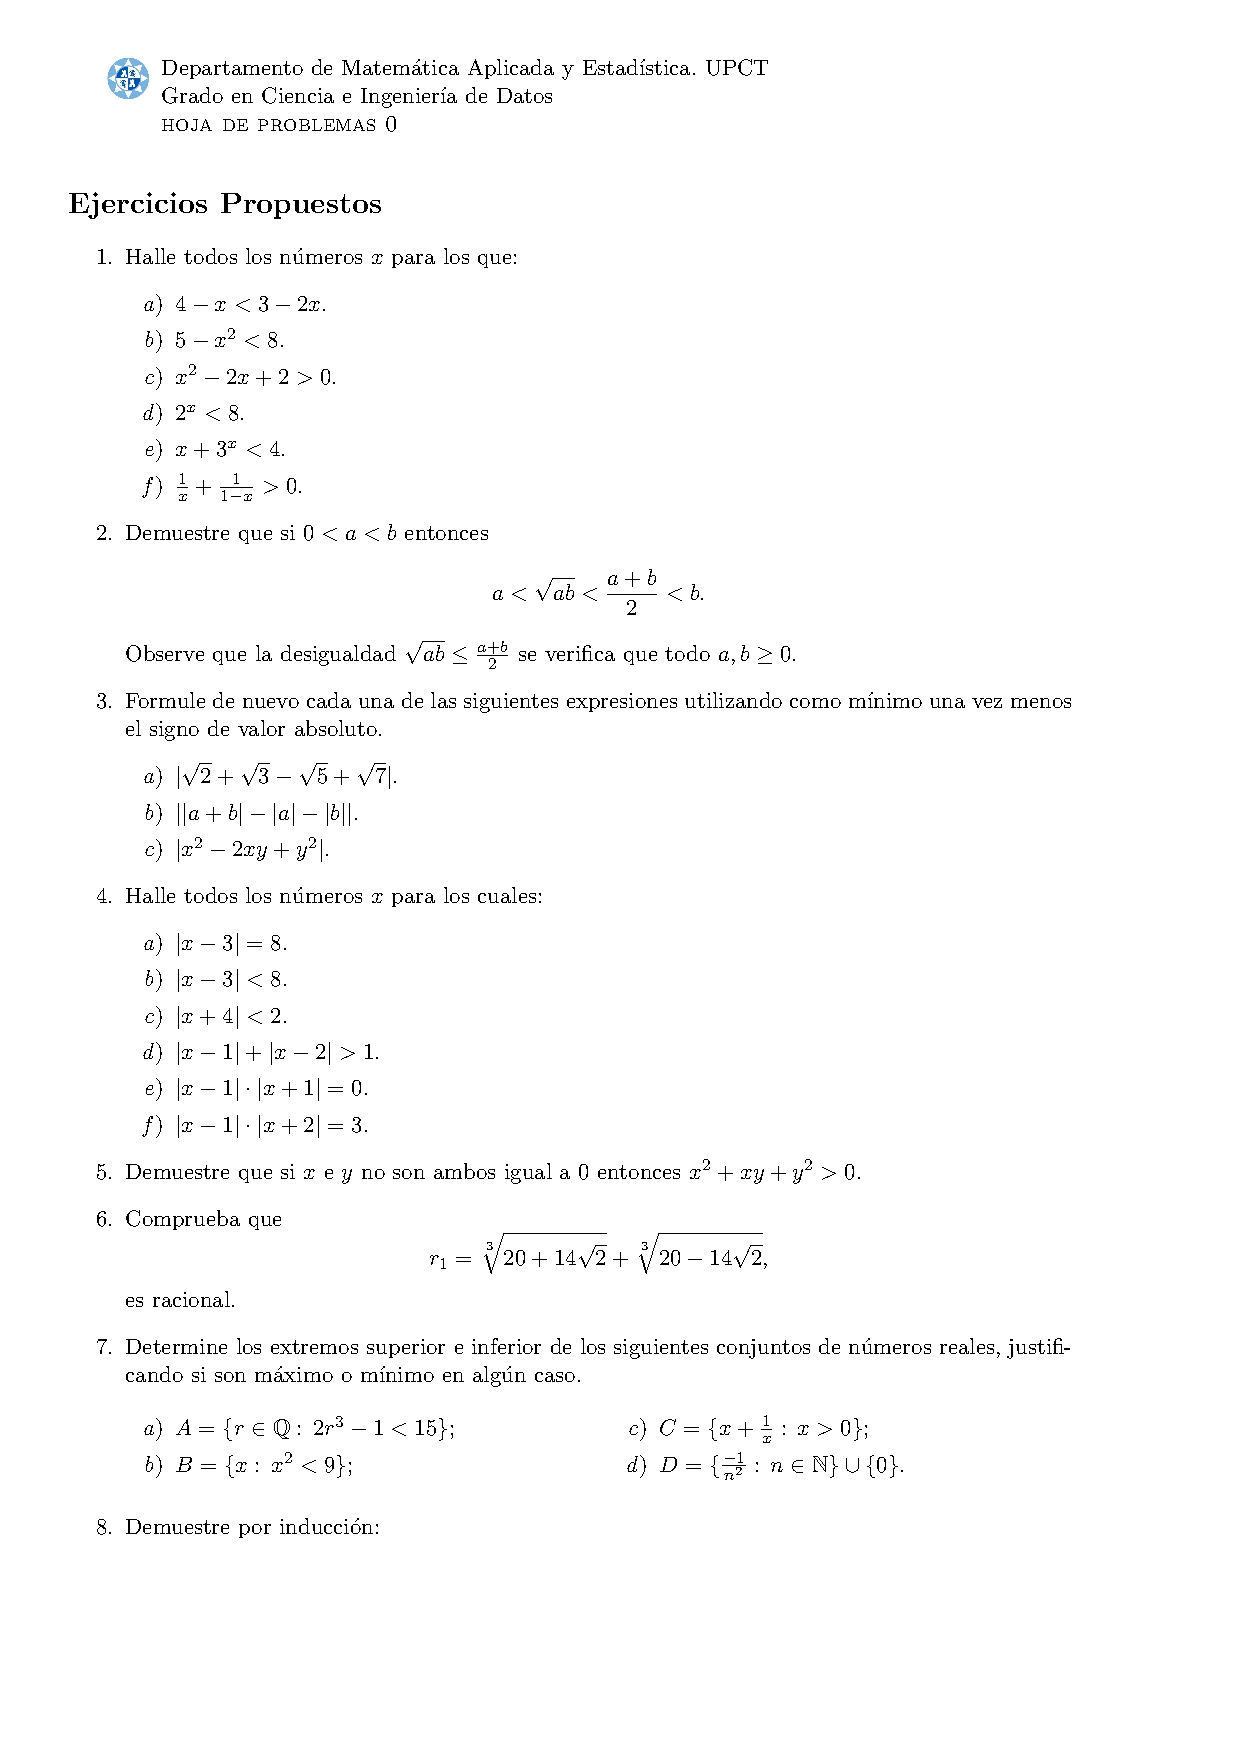
\includepdf[pages=-]{Tema 1/Hoja 1.0/Hoja 0.pdf}

\textcolor{red}{1) }\textcolor{lightblue}{Halle todos los números $x$ para los que:}
\begin{enumerate}[label*=\color{red}\alph*)]
	\item {\color{lightblue} $4-x<3-2x$}
	
	$4-x<3-2x\longrightarrow 2x-x<3-4\longrightarrow x<-1$
	
	\item {\color{lightblue} $5-x^2<8$}
	
	$5-x^2<8\longrightarrow-x^2<8-5\longrightarrow x^2>3\longrightarrow x>\sqrt{3}$
	
	\item {\color{lightblue} $x^2-2x+2>0$}
	
	$\cancel{x=\dfrac{2\pm\sqrt{(-2)^2-4\cdot1\cdot2}}{2\cdot1}=\dfrac{2\pm\sqrt{4-8}}{2}=\dfrac{2\pm\sqrt{-4}}{2}\longrightarrow \nexists x\in\mathbb{R}}$ 
	
	$f'(x)=2x-2\longrightarrow x=\dfrac{2}{2}=1$
	
	Con esto determinamos que $x>0~\forall x\in(-\infty, 1)\cup(1,+\infty)$ siendo $x=1$ su punto crítico.
	
	\item {\color{lightblue} $2^x<8$}
	
	$2^x<8\longrightarrow\log_28=3$
	\begin{tikzpicture}[baseline=(current bounding box.center)]% function
		\begin{axis}[xlabel=x,ylabel=y, ymin=-1, xmin=-1, ymax=8.3,axis lines=center]
			\addplot[lightblue, samples=150, domain=-1:2.99] {2^x};
			\addplot[lightblue] {8};
		\end{axis}
	\end{tikzpicture}
		
	\item {\color{lightblue} $x+2^x<4$}
	
	$\begin{array}{l}
		x+3^x<4\\
		1+3^1=4
	\end{array}$
	\begin{tikzpicture}[baseline=(current bounding box.center)]% function
		\begin{axis}[ymin=-2, xmin=-4, xmax=4, ymax=4.5, axis lines=center]
			\addplot[lightblue, domain=-4:3.9,samples=150] {x+3^x};
			\addplot[lightblue, ] {4};
		\end{axis}
	\end{tikzpicture}
	
	\item {\color{lightblue} $\dfrac{1}{x}+\dfrac{1}{1-x}>0$}
	
	$\dfrac{1}{x}+\dfrac{1}{1-x}=\dfrac{(1-x)+x}{x(1-x)}=\dfrac{1-\cancel{x}+\cancel{x}}{x(1-x)}=\dfrac{1}{x-x^2}\cdot\dfrac{x+x^2}{x+x^2}=$
\end{enumerate}

\textcolor{red}{2) }\textcolor{lightblue}{Demuestre que si $0<a<b$ entonces \[ a<\sqrt{ab}<\dfrac{a+b}{2}<b. \] Observe que la desigualdad $\sqrt{ab}<\dfrac{a+b}{2}$ se verifica que todo $a,b\ge0$.}

\textcolor{red}{3) }\textcolor{lightblue}{Formule de nuevo cada una de las siguientes expresiones utilizando como mínimo una vez el signo de valor absoluto.}

\begin{enumerate}[label=\color{red}\alph*)]
	\item \textcolor{blue}{$|\sqrt{2}+\sqrt{3}-\sqrt{5}+\sqrt{7}|$}
	
	
	
	\item \textcolor{blue}{$\left||a+b|-|a|-|b|\right|$}
	
	
	
	\item \textcolor{blue}{$|x^2-2xy+y^2|$}
	
	
\end{enumerate}

\textcolor{red}{4) }\textcolor{lightblue}{Halle todos los números $x$ para los cuales:}

\begin{enumerate}[label=\color{red}\alph*)]
	\item \textcolor{blue}{$|x-3|=8$}
	
	

	\item \textcolor{blue}{$|x-3|<8$}
	
	
	
	\item \textcolor{blue}{$|x+4|<2$}
	
	
	
	\item \textcolor{blue}{$|x-1|\dot|x-2|>1$}
	
	
	
	\item \textcolor{blue}{$|x-1|\cdot|x+1|=0$}
	
	
	
	\item \textcolor{blue}{$|x-1|\cdot|x+2|=3$}
	
	
\end{enumerate}
\textcolor{red}{5) }\textcolor{lightblue}{Demuestre que si $x$ e $y$ no son ambos igual a 0 entonces $x^2+xy+y^2>0$.}

\textcolor{red}{6) }\textcolor{lightblue}{Comprueba que \[ r_1=\sqrt[3]{20+14\sqrt{2}}+\sqrt[3]{20-14\sqrt{2}}, \] es racional.}

\begin{align*}
	r_1^3 &=(20+14\sqrt{2})+3\left(\sqrt[3]{20+14\sqrt{2}}\right)^2\cdot\sqrt[3]{20-14\sqrt{2}}+3\sqrt[3]{20+14\sqrt{2}}\cdot\left(\sqrt[3]{20-14\sqrt{2}}\right)^2+(20-14\sqrt{2}) \\
	&= 40+3\sqrt[3]{20+14\sqrt{2}}\cdot\sqrt[3]{20^2-2\cdot14^2}+3\sqrt[3]{20-14\sqrt{2}}\cdot\sqrt[3]{20^2-2\cdot14^2}\\
	&=40+3\cdot\sqrt[3]{8}\cdot\sqrt[3]{20+14\sqrt{2}}+3\cdot\sqrt[3]{8}\cdot\sqrt[3]{20-14\sqrt{2}}\\
	&=40+6\cdot\left(\sqrt[3]{20+14\sqrt{2}}+\sqrt[3]{20-14\sqrt{2}}\right)\\
	&=40+6\cdot r_1
\end{align*}